\section{Introduction} 

\begin{figure}[t] \begin{center}
    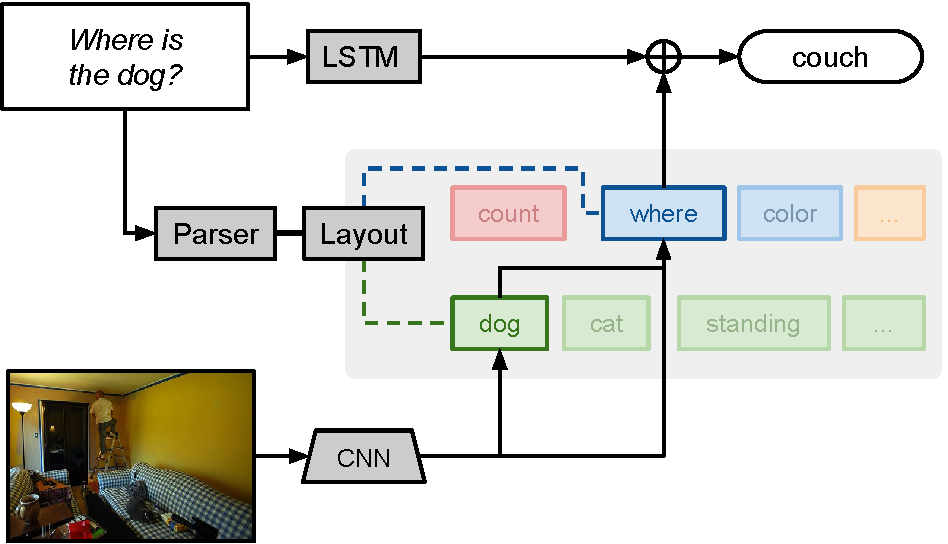
\includegraphics[width=\linewidth]{fig/teaser} \end{center} \caption{
      A schematic representation of our proposed model---the shaded gray area is a
      {\it neural module network} of the kind introduced in this paper. Our
      approach uses a natural language parser to dynamically lay out a deep
      network composed of reusable modules. For visual question answering tasks,
      an additional sequence model provides sentence context and learns
      common-sense knowledge.
    } \label{fig:teaser}
\end{figure}

This paper describes a framework for answering natural language questions with
collections of jointly-trained neural ``modules'', using linguistic structure to
dynamically assemble these modules into deep networks. Our initial focus is on
visual question answering, a task with significant applications to human-robot
interaction, search, and accessibility. Visual QA is the subject of a great deal
of current research attention 
\cite{antol15iccv,gao2015you,ma15arxiv,malinowski15iccv,ren2015image,yu15arxiv}, 
requiring sophisticated understanding of both visual scenes and natural
language.

Specifically, given an image and an associated question (e.g.\ \emph{where is
the dog?}), we wish to predict a corresponding answer (e.g.\ \emph{on the couch},
or perhaps just \emph{couch}). Recent successful represent questions as
bag-of-words \cite{} or read in the question using a single neural network
\cite{malinowski15iccv}\cite{} and train a classifier on the full question
representation and the full-image representation. In contrast to these
monolithic approaches, another line of work for textual QA \cite{Liang13DCS} and
image QA \cite{malinowski14nips} uses semantic parsers to decompose questions
into logical expressions. These logical expressions are evaluated against a
logical representation of the world, which may be provided directly or extracted
from an image \cite{Krish2013Grounded}.

In this paper we draw from both lines of research, presenting a technique for
integrating the representational power of neural networks with the flexible
compositional structure afforded by symbolic approaches to semantics.  Rather
than relying on a monolithic network structure to answer all questions, our
approach assembles a network on the fly from a collection of specialized,
jointly-learned modules (\autoref{fig:teaser}). In particular, we first analyze
the question with an off-the-shelf semantic parser, and use this analysis to
determine the basic computational units (attention, classification, etc.) needed
to answer the question, as well as the relationships between them. In
\autoref{fig:teaser}, we first produce an attention focused on the dog, which sends its output to
a location classifier. Depending on the underlying structure, these messages
passed between modules may be raw image features, attentions, or classification
decisions; each module is determined by its input and output types.
Different kinds of modules are marked with different
colors in \Figref{fig:teaser}: for example the \mod{attend[$dog$]} module
(green) produces a spatial heatmap while the \mod{classify[$where$]} (blue)
recognizes what is in the image region localized by the attention heatmap.
Importantly, all modules of a NMN are independent, which allows the computation
to be different for each problem instance, and possibly unobserved during
training. 
%So that we can answer novel question at test time, such as
%\emph{Where is the banana?}, even we only saw \emph{count} or
%\emph{color} question about \emph{bananas} during training.  
In addition to the NMN our final answer also incorporates the image scene
knowledge (using a full frame CNN) and uses an  recurrent network (LSTM) to read
the question, which has been shown to be important to model common sense
knowledge and dataset biases \cite{malinowski15iccv}.

%Where previous work has
%treated both the image and the question as inputs to a monolithic
%classification model, we instead take the perspective that a question is a
%noisy specification of a hidden computation that must be performed on the image
%to produce an answer. Crucially, this computation may be different for each
%problem instance, and is never observed observed during training.

%Our approach bears a superficial resemblance to a classical semantic parser.
%However, instead of mapping from questions to logical forms, our model maps
%from questions to neural network structures. These networks are assembled on
%the fly (possibly into novel topologies) from a collection of jointly-learned
%neural ``modules''. Finally, they are evaluated against the input image to
%produce an answer.




%This paper presents a technique for following natural language instructions
%(and performing other dynamically-specified tasks) by assembling deep neural
%networks on the fly from an inventory of pre-trained components.

We evaluate our approach on three visual question answering tasks. On the
recently-released CocoQA \cite{yu15arxiv} and  VQA \cite{antol15iccv} datasets,
we achieve results comparable to [better than] existing approaches, and show
that our approach specifically outperforms previous work on questions with
compositional structure (\eg requiring that an object be located and one of its
attributes described). Using our model on questions where compositional
structure plays a central role, and falling back to previous approaches
elsewhere, we achieve new state-of-the-art results on both tasks. It turns out,
however, that most of the questions in both datasets are quite simple, with
little composition. To test our approach's ability to handle highly structured
questions, we introduce a new dataset of synthetic images paired with complex
questions involving spatial relations, set-theoretic reasoning, and shape and
attribute recognition. On this dataset we outperform the previous state of the
art by XXX.

While all the applications considered in this paper involve visual question
answering, the general architecture is potentially of broader usefulness, and
might be more generally applied to referring expression resolution (XXX),
question answering about natural language texts (XXX), or XXX.

%We evaluate our approach on two visual question answering tasks. First we
%present a new synthetic image dataset paired with a complex set of queries
%(involving spatial relations, logical operators, and shape and attribute
%recognition). Next, we consider a hard subset of the Microsoft VQA corpus of
%questions about natural images. In each case, an NMN-based approach outperforms
%state-of-the-art models with more conventional recurrent architectures. We
%observe in particular that NMNs are able to make considerably better use of
%small training sets.

To summarize our contributions: We first propose neural module networks, a
general architecture for discretely composing heterogeneous, jointly-trained
neural modules into deep networks. Next, for the visual QA task specifically, we
show how to construct NMNs based on the output of a semantic parser, and use
these to successfully complete established visual question answering tasks.
Finally, we introduce a new dataset of challenging, highly compositional
questions about abstract shapes, and show that our approach outperforms previous
models by as much as XXX. We will release this dataset, as well as code for all
systems described in this paper upon publication.

\section{Motivations}

%Many tasks in computer vision, including recognition, detection, and captioning,
%share common substructure. For example, we might schematically express the
%sequence of computations performed by a recognizer as
%\begin{flushleft}
%  \mod{classify(pickMostRelevant(detectObjects))}
%\end{flushleft}
%or a detector as
%\begin{flushleft}
%  \mod{drawBoundaries(detectObjects)}
%\end{flushleft}
%
%In practice the picture is not this clean---classification or detection is
%performed end-to-end by a single neural network, and the boundaries between
%these ``phases'' are not clearly defined. Nevertheless we might expect \textit{a
%priori} that a network used for classification might expose intermediate
%representations useful for building a detector. 
We begin with two simple observations. First, that there is no single ``best
network'' for all purposes---state-of-the-art performance on the full range of
computer vision tasks that are studied requires a variety of different deep
network topologies. Second, though different networks are used for different
purposes, it is commonplace to initialize systems for many of vision tasks with
a prefix of a network trained for classification \cite{Long14FullyConvolutional} XXX. 
This has been shown to substantially reduce training time and improve accuracy. 

So while network structures are not \emph{universal} (in the sense that the same
network is appropriate for all problems), they are at least empirically
\emph{modular} (in the sense that intermediate representations for one task are
useful for many others). 

Can we generalize this idea in a way that is useful for question answering?
Rather than thinking of question answering as a problem of learning a single
function to map from questions and contexts to answers, it's perhaps useful to
think of it as a highly-multitask learning setting, where each problem instance
is associated with a novel task, and the identity of that task is expressed only
noisily in language. In particular, where a simple question like \emph{is this a
truck?} requires us to retrieve only one piece of information from an image,
more complicated questions, like \emph{how many objects are to the left of
the toaster?} might require multiple processing steps. The compositional nature
of language (XXX) means that the number of processing such steps is potentially
unbounded. Moreover, multiple \emph{kinds} of processing might be
required---repeated convolutions might identify a truck, but some kind of
recurrent architecture is likely necessary to count up to arbitrary numbers.

Thus our goal in this paper is to specify a framework for modular, composable,
jointly-trained neural networks. In this framework, we first predict the
structure of the computation needed to answer each question individually, then
realize this structure by constructing an appropriately-shaped neural network
from an inventory of reusable modules. These modules are learned jointly, rather
than trained in isolation, and specialization to individual tasks (identifying
properties, spatial relations, etc.) arises naturally from the training
objective.

%If we consider a few examples of questions:
%XXX
%\begin{center}
%  \begin{tabular}{ll}
%    {\it how many black cats?} & \mod{count(and(detect[cat], detect[black]))} \\
%    {\it what color is the cat?} & \mod{classify[color](detect[cat])} \\
%    {\it what color is the dog?} & \mod{classify[color](detect[dog])} \\
%    {\it is there a dog?} & \mod{exists(detect[dog])}
%  \end{tabular}
%\end{center}
%we again see that there is common computational substructure involved in solving
%the associated tasks.  With sub-networks for computing \mod{detect[cat]},
%\mod{classify}, \mod{count}, etc., we can in principle answer
%questions with novel structure like---e.g.\ {\it is there a black
%dog?}---without any additional training data.
%
%Note in particular that we expect these modules to differ not only in their
%parameters, but more fundamentally in their topologies. Intuitively,
%\mod{detect[cat]} should take an image as input, perform some
%fully-convolutional operation, and output an attention (understood as a
%distribution over positions in the image), while {\small\tt classify[color]}
%should take both the input image and such an attention, and map to a
%distribution over labels. Some computations require convolutional operations,
%some require fully-connected operations, and some (like counting) may require
%recurrent network structures. We should not expect that we will be able to use
%the same network layout for every problem, but do expect that parts of these
%networks may be reused in different orders.

\section{Related work}

The idea of selecting a different network graph for each input datum is fundamental to both recurrent networks (where the network grows in the length of the input) \cite{Elman90RNN} and recursive neural networks (where the network is built, e.g., according to the syntactic structure of the input) \cite{Socher13CVG}. But both of these approaches ultimately involve repeated application of a single computational module (\eg an LSTM \cite{} or GRU \cite{} cell). Our basic contribution is in allowing the nodes of this graph to perform heterogeneous computations, and for "messages" of different kinds---raw image features, attentions, classification predictions---to be passed from one module to the next. We are unaware of any previous work allowing such mixed collections of modules to be trained jointly. 

\paragraph{non-image QA}
text only based: \cite{berant14acl,Liang13DCS}

\cite{geman15nas} a binary (yes/no) version of Visual Turing Test on synthetic data.

We are also unaware of past use of a semantic parser to predict network structures, or more generally to exploit the natural similarity between set-theoretic approaches to classical semantic parsing and attentional approaches to computer vision. As noted above, there is a large literature on learning to answer questions about structured knowledge representations from question--answer pairs, both with and without learning of meanings for simple predicates \cite{Liang13DCS,Krish2013Grounded}.

``neural'': \cite{iyyer14emnlp,weston14arxiv}

\paragraph{Grounding in images}
Deep Fragments \cite{karpathy14nips}, Flickr30k Entities \cite{plummer15iccv}.
Deep Visual-Semantic Alignments for Generating Image Descriptions \cite{karpathy15cvpr}.
(Image Retrieval using Scene Graphs \cite{johnson15cvpr})

\cite{Krish2013Grounded,matuszek12icml,kong14cvpr}

\paragraph{Datasets}
The present work is made possible by a number of recently-created corpora for question answering about images, including the DAQUAR dataset \cite{malinowski14nips}, the CocoQA dataset \cite{yu15arxiv}, and the VQA dataset \cite{antol15iccv}. 




\paragraph{image QA}
``classical'': \cite{malinowski14nips}

``neural'':
Several models for visual questioning have already been proposed in the literature \cite{ren2015image,ma15arxiv,gao2015you}, all of which use standard deep sequence modeling machinery to construct a joint embedding of image and text, which is immediately mapped to a distribution over answers. Here we attempt to more XXXly model the computational process needed to produce each answer, but also benefit from sequence and image embeddings XXX.


\section{Neural module networks for visual QA}

%Given a pre-trained \emph{network layout predictor} $P$, 
each training datum for this task can be thought of as a 4-tuple $(w, x, y)$, where
\begin{itemize}
  \setlength\itemsep{0em}
  \item $w$ is a natural-language question
  %\item $p = P(w)$ a network layout
  \item $x$ is an image
  \item $y$ is an answer
\end{itemize}
A model is fully specified by a collection of modules $\{ m \}$, each with
associated parameters $\theta_m$. Given $(w, x)$ as above, the model
instantiates a network based on $w$, passes $x$ (and possibly $w$ again) as
inputs, and obtains a distribution over labels (for the VQA task, we require the
output module to be a classifier). Thus a model corresponds to a predictive
distribution $p(y\ |\ w, x; \theta)$.

In the remainder of this section, we first describe the set of modules used for
the VQA task, then explain the process by which questions are converted to
network layouts.

\subsection{Modules}

Our goal in this section is to identify a small set of modules that can be
assembled into all the configurations necessary for our tasks. This corresponds
to identifying a minimal set of composable vision primitives. The modules
operate on three basic data types: images, unnormalized attentions, and labels.
For the particular task and modules described in this paper, almost all
interesting compositional phenomena occur in the space of attentions, and it is
not unreasonable to characterize our contribution more narrowly as an
``attention-composition'' network. Nevertheless, other types may be
required in the future (for different new or for greater coverage in the VQA
domain).

First, some notation: module names are typeset in a {\tt fixed width font}, and
are of the form \mod{TYPE[INSTANCE](ARG$_1$, \ldots)}. \mod{TYPE} is a
high-level module type (attention, classification, etc.) of the kind described
in this section. \mod{INSTANCE} is the particular instance of the model under
consideration---for example, \mod{attend[red]} locates red things, while
\mod{attend[dog]} locates dogs. Weights may be shared at both the type and
instance level. Modules with no arguments implicitly take the image as input;
higher-level arguments may also inspect the image.

\[
  \mod{attend} : \mathit{Image} \to \mathit{Attention}
\]
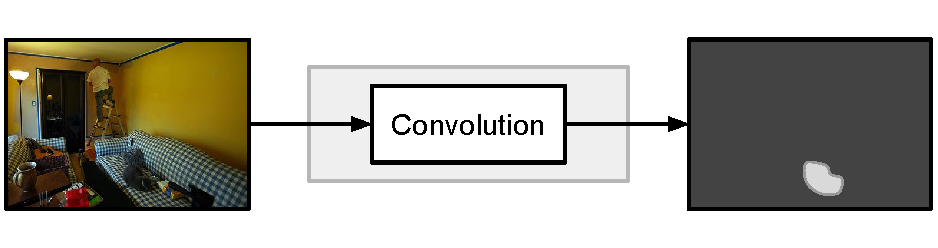
\includegraphics[width=\columnwidth]{fig/attend}
An attention module \mod{attend[$c$]} convolves every position in the input
image with a weight vector (distinct for each $c$) to produce a heatmap or
unnormalized attention. So, for example, the output of the module {\small\tt
attend[dog]} is a matrix whose entries should be in regions of the image
containing cats, and small everywhere else, as shown above.\\

\[
  \mod{re-attend} : \mathit{Attention} \to \mathit{Attention}
\]
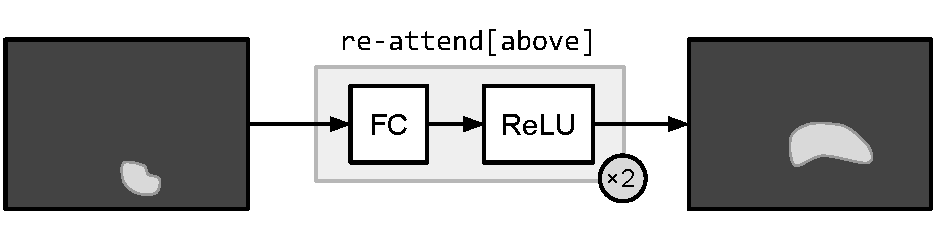
\includegraphics[width=\columnwidth]{fig/re-attend}
A re-attention module \mod{re-attend[$c$]} performs a fully-connected mapping
from one attention to another. Again, the weights for this mapping are distinct
for each $c$. So \mod{re-attend[above]} should take an attention and shift the
regions of greatest activation upward (as above), while \mod{re-attend[not]}
should move attention away from the active regions.\\%[1em]

\[
  \mod{combine} : \mathit{Attention} \times \mathit{Attention} \to
  \mathit{Attention}
\]
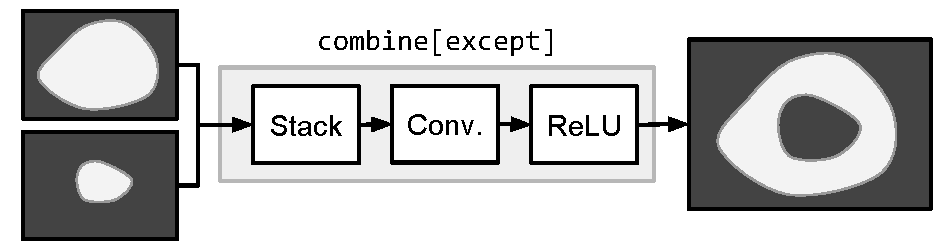
\includegraphics[width=\columnwidth]{fig/combine}
A combination module \mod{combine[$c$]} merges two attentions into a single
attention. For example, {\small\tt combine[and]} should be active only in the
regions that are active in both inputs, while {\small\tt{combine[except]}}
should be active where the first input is active and the second is
inactive.\\[1em] 

\[
  \mod{classify} : \mathit{Image} \times \mathit{Attention} \to
  \mathit{Label}
\]
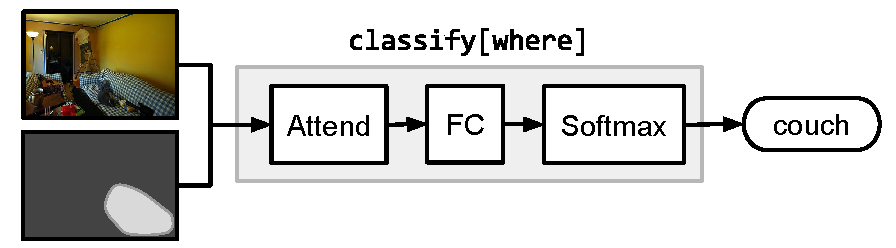
\includegraphics[width=\columnwidth]{fig/classify}
A classification module \mod{classify[$c$]} takes an attention and the input
image and maps them to a distribution over labels. For example, {\small\tt
classify[color]} should return a distribution over colors for the region
attended to.\\[1em]

\[
  \mod{measure} : \mathit{Attention} \to \mathit{Label}
\]
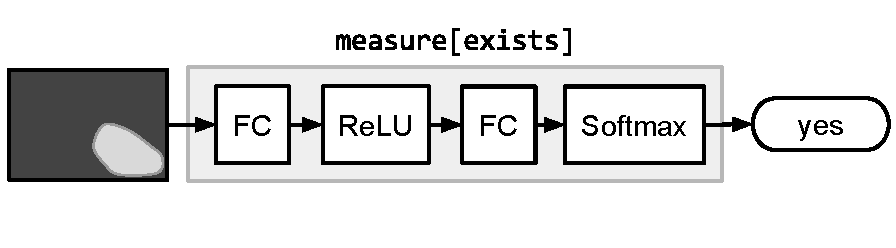
\includegraphics[width=\columnwidth]{fig/measure}
A measurement module \mod{measure[$c$]} takes an attention alone and maps it to
a distribution over labels. Because attentions passed between modules are
unnormalized, \mod{measure} is suitable for evaluating the existence of a
detected object, or counting sets of objects.

\subsection{From strings to networks}

In this section, we first describe how to map from natural language questions to
\emph{layouts}, which specify both the set of modules used to answer a given
question, and the connections between them. Next we describe how layouts are
used to assemble the final prediction networks.

To predict layouts use standard tools pre-trained on existing linguistic
resources to obtained structured representations of questions. Future work might
focus on learning (or at least fine-tuning) this prediction process jointly with
the rest of the system, though in fact off-the-shelf tools produce high-quality
analyses for almost all the questions in our data.

\paragraph{Parsing}
Specifically, we begin by parsing each question with the Stanford Parser (XXX)
to obtain a universal dependency representation (XXX). Dependency parses express
grammatical relations between parts of a sentence (e.g.\ between objects and
their attributes, or events and their participants), and provide a lightweight
abstraction away from the surface form of the sentence. The parser also performs
basic lemmatization, for example turning \emph{kites} into \emph{kite} and
\emph{were} into \emph{be}. 

Next, we filter the set of dependencies to those connected the wh-word in the
question (the exact distance we traverse varies depending on the task). This
gives a simple logical form expressing (the primary) part of the sentence's
meaning.  For example, \emph{what is standing in the field} becomes
\mod{what(stand)}; \emph{what color is the truck} becomes \mod{color(truck)},
and \emph{is there a circle next to a square} becomes \mod{is(cicle,
next-to(square))}.
In the process we also strip away function words like determiners and
modals, so \emph{what type of cakes were they?} and \emph{what type of cake is
it?} both get converted to \mod{type(cake)}.

It is easiest to think of these representations as pieces of a variable-free
combinatory logic \cite{Liang13DCS}; every leaf is implicitly a function taking
the image as input. The code for transforming parse trees to structured queries
will be provided in the accompanying software package.

\paragraph{Layout}
These logical forms already determine the structure of the predicted network,
but not the identities of the modules that compose it. This final assignment of
modules is fully determined by the structure of the parse. All leaves become
\mod{attend} modules, all internal nodes become \mod{re-attend} or \mod{combine}
modules dependint on their arity, and root nodes become \mod{measure} modules
for yes/no questions and \mod{classify} modules for all other quesiton types.

Given the mapping from queries to network layouts described above, we have for
each training example a network structure, an input image, and an output label.
In many cases, these network structures are different, but have tied parameters.
Networks which have the same high-level structure but different instantiations
of individual modules (for example \emph{what color is the cat?}---{\small\tt
classify[color](attend[cat])} and \emph{where is the truck?}---{\small\tt
classify[where](attend[truck])}) can be processed in the same batch, resulting
in efficient computation.

As noted above, parts of this conversion process are task-specific---we found
that relatively simple expressions were best for the natural image questions,
while the shapes question (by design) required deeper structures. Some summary
statistics are provided in Table XXX.

\begin{table*}
  \centering
  \begin{tabular}{cccccc}
    \toprule
    & \# types & \# instances & \# layouts & Max depth & Max size \\
    \midrule
    VQA & 4 & 1995 & 66549 & 2 & 3 \\
    \cocoqa & 3 & 892 & 4613 & 2 & 2\\
    \shapes & 4 & 8 & 164 & 5 & 6 \\
    \bottomrule
  \end{tabular}
  \caption{Structure summary statistics for neural module networks used in this
    paper. ``\# types'' is the number of high-level module types available (e.g.
    \emph{attend}), ``\# instances'' is the number of specific module instances
    (e.g. \mod{attend[llama]}), and ``\# layouts'' is the number of distinct
    composed structures (e.g. \mod{classify[color](attend[llama])}).
    ``Max depth'' is the greatest depth across all layouts, while ``max
    size'' is the greatest number of modules---the network in XXX has depth 4
    and size 5.
    (All numbers from training sets.)
  }
\end{table*}

\paragraph{Generalizations}

It is easy to imagine applications where the input to the layout stage comes
from something other than a natural language parser. Users of an image database,
for example, might write SQL-like queries directly in order to specify their
requirements precisely, e.g.
\begin{flushleft}
  {\tt IS(cat) AND NOT(IS(dog))}
\end{flushleft}
or even mix visual and non-visual specifications in their queries:
\begin{flushleft}
  {\tt IS(cat) and date > 2014-11-5}
\end{flushleft}

Indeed, it is possible to construct this kind of ``visual SQL'' using exactly
the models learned in this paper---once our system is trained, the learned
modules for attention, classification, etc. can be assembled by any kind of
outside user, without relying on natural language specifically.

\begin{figure*}
  \begin{subfigure}[t]{0.4\textwidth}
    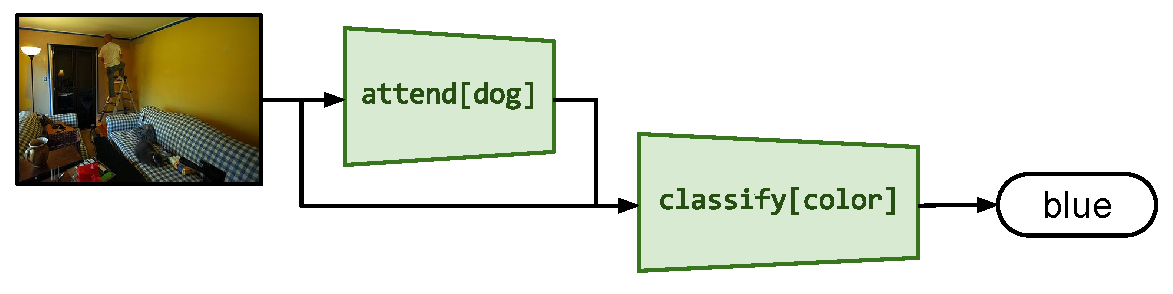
\includegraphics[width=\textwidth]{fig/full1}
    \caption{NMN for answering the question \emph{What color is
    his tie?} The \mod{attend[tie]} module first predicts a heatmap
    corresponding to the location of the tie. Next, the \mod{classify[color]}
    module uses this heatmap to produce a weighted average of image features,
  which are finally used to predict an output label.}
  \end{subfigure}
  \hfill
  \begin{subfigure}[t]{0.55\textwidth}
    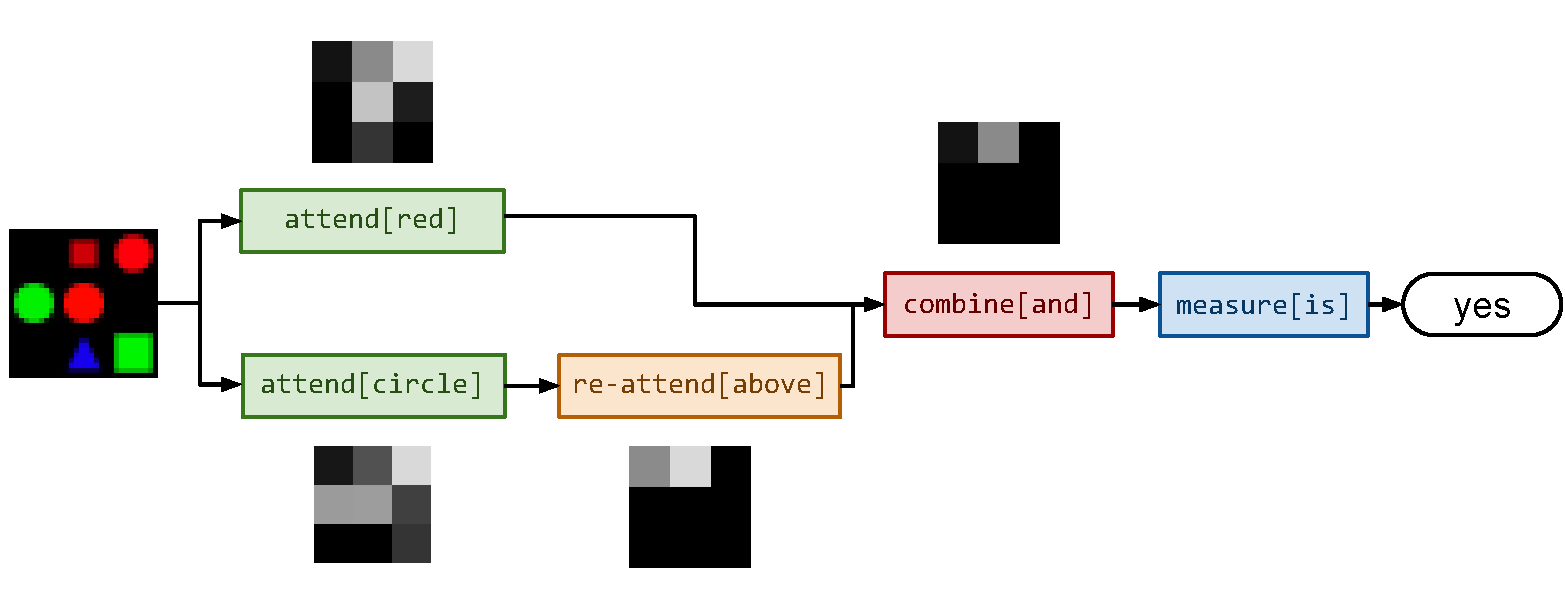
\includegraphics[width=\textwidth]{fig/full2}
    \caption{NMN for answering the question \emph{Is there a red shape above a
    circle?} The two \mod{attend} modules locate the red shapes and circles,
    the \mod{re-attend[above]} shifts the attention above the circles, the
    \emph{combine} module computes their intersection, and the
    \mod{measure[is]} module inspects the final attention and determines
  that it is non-empty.}
  \end{subfigure}
  \caption{Sample NMNs for question answering about natural images and shapes.
  For both examples, layouts attentions and answers are real predictions made by
  our model.}
\end{figure*}

\section{Training neural module networks}

Our training objective is simply to find module parameters maximizing the
likelihood of the data. By design, the last module in every network is a
{\small\tt classify}, and so each assembled network represents a probability
distribution.

Because of the dynamic network structures used to answer questions, some weights
are updated much more frequently than others. For this reason we found that
learning algorithms with adaptive per-weight learning rates performed
substantially better than simple gradient descent. All the experiments described
below use AdaDelta (XXX) (thus there was no hyperparameter search over step
sizes).

It is important to emphasize that the labels we have assigned to distinguish
instances of the same module type---\mod{cat}, \mod{and}, etc.---are a
notational convenience, and do not reflect any manual specification of the
behavior of the corresponding modules. \mod{detect[cat]} doesn't know it's
supposed to be a cat recognizer (rather than a couch recognizer or a dog
recognizer),
and \mod{combine[and]} doesn't know it's supposed to compute intersections of
attentions (rather than unions or differences). Instead, they acquire these
behaviors as a byproduct of the end-to-end training procedure. As can be seen in
Figure XXX, the image--answer pairs and parameter tying together encourage each
module to specialize in the appropriate way.


